\documentclass[letterpaper,12pt]{article}
\usepackage[utf8]{inputenc}
\usepackage[english]{babel}
\usepackage[margin=1in]{geometry}
\usepackage{graphicx}
\usepackage[printonlyused]{acronym}
\usepackage{tikz}
\usepackage{wrapfig}
\usepackage{lscape}
\usepackage{hyperref}
\usepackage{rotating}
\usepackage{epstopdf}
\usepackage{setspace}
\usepackage[labelfont=bf]{caption}
\usepackage[tocgraduated]{tocstyle}
\widowpenalty10000
\clubpenalty10000
\usetocstyle{allwithdot}
\renewcommand*\contentsname{Table of Contents}
\usepackage[
    backend=biber,
    style=numeric,
    sorting=ynt
    ]{biblatex}
\addbibresource{references.bib}
\setlength{\parindent}{4em}
\graphicspath{{./images/}}


\usepackage[utf8]{inputenc}
\usepackage[english]{babel}
\usepackage[margin=1in]{geometry}
\usepackage{graphicx}
\usepackage[printonlyused]{acronym}
\usepackage{tikz}
\usepackage{wrapfig}
\usepackage{lscape}
\usepackage{rotating}
\usepackage{epstopdf}
\usepackage{setspace}
\definecolor{rfc}{RGB}{153,102,255}
\definecolor{land}{RGB}{88,74,72}
\definecolor{ada}{RGB}{46,111,211}
\definecolor{grad}{RGB}{22,101,105}
\definecolor{qda}{RGB}{179,179,179}
\definecolor{dtc}{RGB}{46,211,72}
\definecolor{voting}{RGB}{204,204,0}
\definecolor{bag}{RGB}{255,127,72}
\definecolor{mlp}{RGB}{255,66,66}
\definecolor{knn}{RGB}{51,102,0}
\definecolor{gau}{RGB}{153,51,51}
\usepackage[
    backend=biber,
    style=alphabetic,
    sorting=ynt
    ]{biblatex}
\addbibresource{references.bib}
\graphicspath{{./images/}}

\doublespacing
\begin{document}
% Use the following at camera-ready time to suppress page numbers.
% Comment it out when you first submit the paper for review.
%\thispagestyle{empty}arg
    \title{Experimenting with Model Selection for Predicting Global Bathymetry using Machine Learning}
    \author{Nicholas Moran}
    \date{05-25-2020}
    \maketitle
    \section{Abstract}
\setlength{\parindent}{10ex}
This work is concerned with the viability of \ac{ML} for training models  for predicting global bathymetry, and whether there is a best fit model for predicting that bathymetry.
The desired result is a investigation of the ability for \ac{ML} to be used in future prediction models, and experimenting with multiple trained models to determine a optimumum selection.
Ocean features were aggregated from a set of external studies and placed into \~{}2 minute spatial grids representing Earth's oceans.
A set of regression models, classification models, and a novel classification model were then fit to this data and analyzed.
The novel classification model is optimized by selecting the best performing model in a geospatial area.
This optimization increases prediction accuracy for test purposes by approximately 3\%.
Training these models was performed using bathymetry data from the ETOPO2v2 dataset.
While analysis of each utilized the bathymetry from the ETOPO dataset, and subsequent metrics were produced and reported.
Results demonstrate that ocean features can potentially be used to build a prediction model for bathymetry with the inclusion of accurate data and intelligent model selection.
Based on the results in this work, there is evidence that no single model will best predict all Global bathymetry.

    
%Here is what I am about to tell you in this paper. Fairly informal and loose.
\section{Introduction}
\setlength{\parindent}{10ex}
The most accurate world bathymetry mappings come from a aggregate of predicted and measured sources. 
Earth Gravitational Models (EGM) are popularly used for predicting bathymetry \cite{becker2009global}\cite{smith1994bathymetric}\cite{smith1997global}\cite{smith2010planning}.
While sonar platforms such as the Multi Beam Echo Sonar (MBES) \cite{farr1980multibeam} are used for accurate measurements of the bathymetry.
Naturaly, it is not cost and time effective to collect large swaths of MBES bathymetry measurements.
EGMs use sattelite altimeter data to create gravitational models for predicting geoids.
In general, these models predict bathymetry with a error of 190 meters \cite{jena2012prediction}.

\par
There has been much work on using sattelite altimeter derived gravity to predict bathymetry.
This work focuses on using ocean features derived from other studies as predictors.
The goal being to create a model that can predict bathymetry using other features than gravity.
In this work I introduce an approach for optimizing model selection, feature selection, and a novel approach to predicting bathymetry.
    \section{Literature Review}
\setlength{\parindent}{10ex}
In this review different approaches for predicting bathymetry are discussed.
The two main methods for collecting bathymetry data are \ac{SDB} and \ac{EGM}.
There is also a third approach discussed that improves upon the idea of a \ac{EGM}.
\ac{MBES} for precise measurements of bathymetry \cite{farr1980multibeam} is also covered.

\subsection{Machine Learning}
Machine Learning can be defined as the process of fitting a model to data with a algorithm \cite{bishop2006pattern}.
Predictions can then be produced from the models by supplying new data.
To validate the predictions, the supplied data's result is known.
For example, a model is trained to predict if a image contains a car.
Data from the images are extracted and used to train the model.
Images with cars can be considered positive images.
Images with out cars can be considered negative images.
New images that are labeled as positive or negative are given to the model for validation.
If the model successfully predicts the labels it will have a high accuracy and be a "valid" model.
The two main types of models in Machine Learning is classification and regression models.
There are several high level descriptions of classification and regression models including: supervised learning, unsupervised learning, and reinforcement learning.

\par
Classification models are models that predict a discrete value.
For example, the car model mentioned earlier.
The model predicts a discrete value of either positive or negative.
These types of models are effective at predicting values that can be grouped into "labeled" data.
Classification models can also be combined to form ensemble models.
A ensemble is a combination of "weaker" predictors to form a strong predictor.
%Include citations BELOW!!!!!
Examples of classification models used in this project include: Decision Trees, Naive Bayes, MLP Classifier, Quadratic Discriminant Analysis Classifier, and K Nearest Neighbors Classifier.
Examples of ensemble classifiers used in this project include: Random Forest Classifier, Ada boost, Gradient Boosting, Bagging, and Voting.

\par
Regression models predict a continuous value.
For example, predicting water depth as a number is a continuous value.
Where the range of predicted values is from sea level to the known depth of the ocean.
Essentially, this model represents a mathematical function where the input data is the function parameters.
This method is best when the desired result can not be grouped into discrete "labeled" data.

\par
Unsupervised learning describes a model that is trained without labels.
Meaning that the data does not have corresponding "ground-truth" values for predictions \cite{bishop2006pattern}.
Training a model without "ground-truth" is used for grouping similar values together pragmatically.
Ideal for identifying correlations in data that is otherwise unrelated and unlabeled.

\par
Supervised learning describes a model that is trained with labels \cite{bishop2006pattern}.
Training is guided or supervised by comparing results to labeled data.
This method of training is effective at fitting accurate models, and is used in this project for predicting bathymetry.
All models trained in this project use supervised learning.
Each model used will be discussed in subsequent sections.

\subsubsection{Bias and Variance}
%Describe the Bias and Variance relationship!
The generalized error of a model can be expressed in terms of bias and variance.
Bias is the average error of a model for different training sets.
Variance describes the sensitivity of the model to data.
These two terms are necessary to understand the bias-variance problem.
This problem applies to all forms of supervised learning \cite{geman1992neural} and describes the indirect relationship of bias and variance.
The relationship being the minimization of bias often causing high variance, and minimizing variance often causing high bias.
Optimally, accurate models should have a low bias and variance.

%Include image showing bias and variance here!!
\begin{figure}[h]
    \centering
    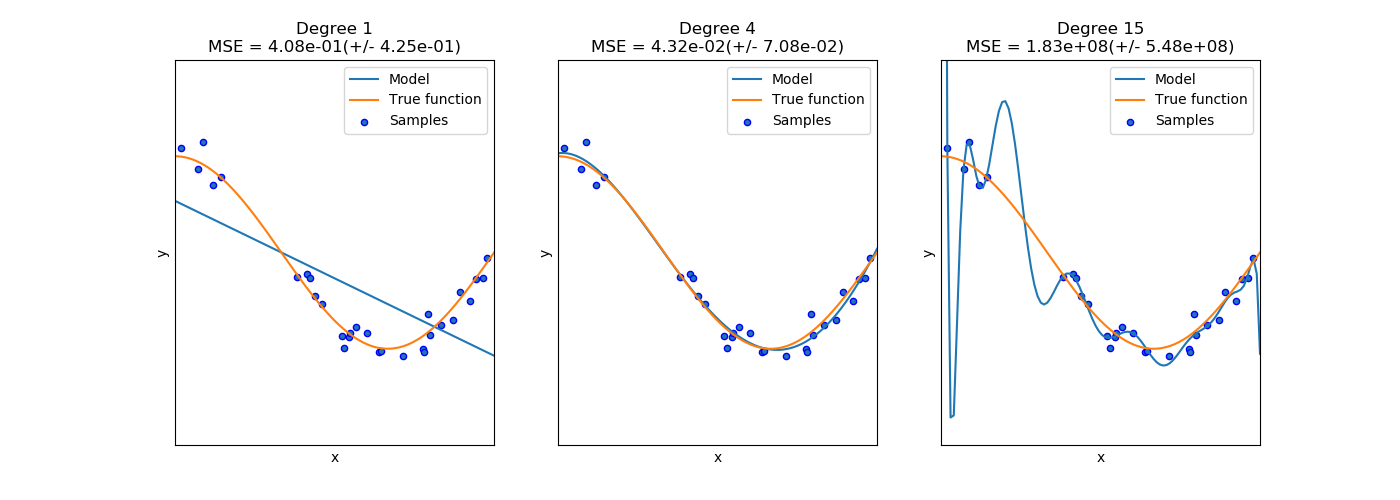
\includegraphics[scale=0.5]{sphx_glr_plot_underfitting_overfitting_001.png}
    \caption{Figure showing Bias and Variance examples}
    \label{}
\end{figure}

\subsubsection{Decision Trees}
%Talk about decision trees here
Decision trees are supervised models that are used for classification or regression \cite{breiman2017classification}.
They are simple to understand and interpret due to their simple decision structure. 
They are susceptible to over fitting and can create overly complex trees that do not generalize well.
Over fitting is where a model will fit to closely to a training set \cite{cawley2010over}. 
Making it unable to make accurate predictions on data outside of what was used in training.

\begin{figure}[h]
    \centering
    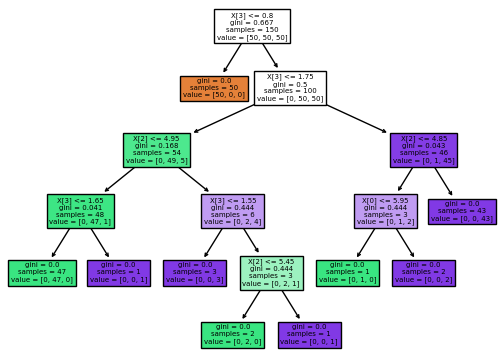
\includegraphics[scale=0.5]{dtreesepal.png}
    \caption{Figure showing example of Decision Tree}
    \label{}
\end{figure}

%Talk about random forest here
\par
The Random Forest Classifier is a ensemble of many decision trees \cite{breiman2001random}.
It fits a number of decision trees on various sub samples of the dataset.
This also helps to control over fitting because each tree is fit to a sub sample of the dataset.
It averages the prediction of each tree to make a more accurate prediction than any single tree.


\subsubsection{Boosting}
%Talk about Ada Boost here
Boosting describes a type of ensemble that is concerned with reducing bias.
The idea being to build base estimators sequentially and then use the results of each to train a different estimator with the intention of reducing bias.
Adaboost is an example of one such model \cite{freund1995desicion}.
Its core principle being the fitting of weak learners on many random samples of the training data.
This learners are then combined with a majority weighted vote. 
This process is iterated for the training phase.



%Talk about Gradient Boosting Here
%Need to finish this paragraph....
\par
The gradient boosting classifier is an ensemble of trees similar to a random forest classifier.
In gradient boosting, decision trees are used as "weak" learners.
They are gradually added to the model in order to reduce the error.
This "gradient decent" approach is effective at building a successful classifier.
These types of boosting algorithms tend to overfed the model.
This can be solved by enforcing tree constraints and random sampling of data.


\subsubsection{Averaging}
Averaging ensembles operate by aggregating the predictions of many models trained on random sub sets of the training data.
Introducing randomization into the training will often reduce the variance of the resulting ensemble.
Bagging is a example of a averaging ensemble and has several implementations.
The Bagging ensemble uses a single classifier and fits instances of it to random samples of the training data.
The predictions are then aggregated and averaged for a final prediction.

%Talk about voting here
The voting classifier works by using the predictions of a set of conceptually different predictors as votes.
The majority vote (hard voting) or averaged vote (soft voting) is selected as the prediction.
This classifier is good for combining equally performing models in order to balance out individual weaknesses.

\subsubsection{K Nearest Neighbors}
%Talk about KNN for classification
The K Nearest Neighbors algorithm is a non-parametric algorithm for classification and regression \cite{altman1992introduction}.
K Nearest Neighbors for classification stores the instances of the training data and associated labels.
Predictions are made by computing the distance of new instances to the training set.

\subsubsection{Multi Layer Perception}
%Talk about MLP Classifier here!!!
% Include MLP picture here I guess
The Multi Layer Perceptron is a model that fits a function iterative through a process called back propagation.
The MLP classifier is a neural network model that is based on the structure of the human brain.
It consists of many layers beginning with an input layer.
The middle layers are called the "hidden layers" and are each assigned a weight.
Back propagation is used during training to adjust the weights in the hidden layers.
These adjustments are made to in order to reach a more accurate prediction.
There can be many hidden layers of different depths.
% Probably need to say more about the MLP Classifier...
% Maybe some graphics and other bull jive. Maybe a algorithm???

\begin{figure}[h]
    \centering
    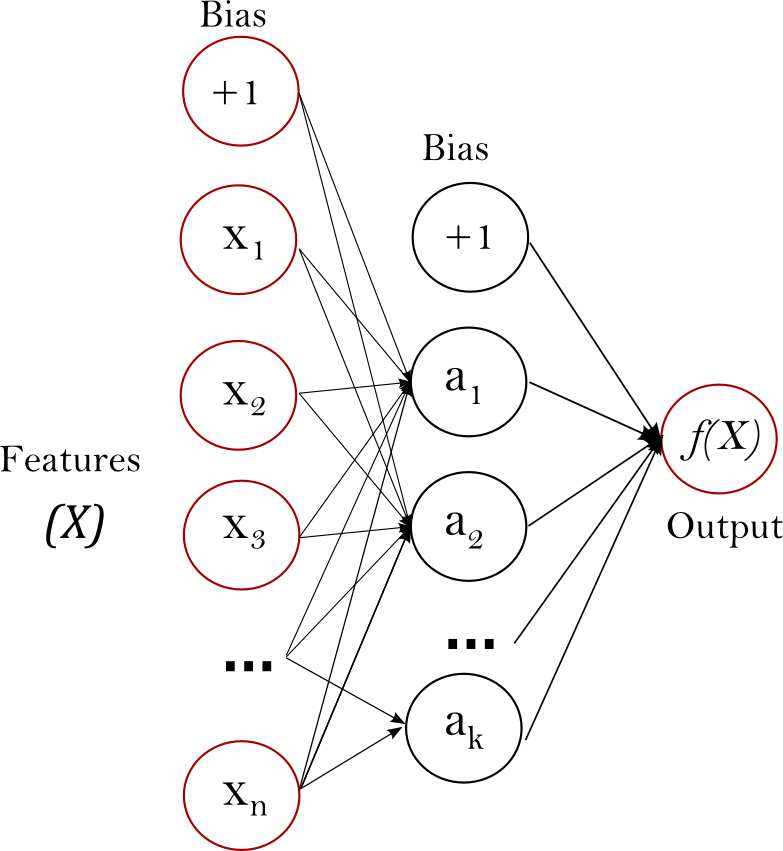
\includegraphics[scale=0.5]{multilayerperceptron_network.png}
    \caption{Figure showing Neural Network Model}
    \label{}
\end{figure}

%include more here about MLP


\subsubsection{Naive Bayes}
%Talk about Naive Bayes classifier here!!
The naive Bayes classifier is based on applying the naive Bayes theorem \cite{zhang2004optimality}.
The naive assumption of Naive Bayes is the conditional independence between pairs of features given the label.
Bayes theorem states the following relationship given class y and feature vector x.

% Put bayes theorem right here!!! Math mode I guess...


\subsubsection{Regression Models}
%Talk about Regression models used here...
Regression models are utilized for predicting continuous values.
Specifically, regression is for approximating a function given a set of inputs to yield a output.
Linear regression is the simplest type and is concerned with fitting a linear combination of all training features.

% Put linear regression equation right here for the world to see YO

This project utilizes three regression models from sci kit.
The naive Bayes\cite{sklearn_api}, logistic regression\cite{sklearn_api}, and svm regression\cite{sklearn_api} models are utilized for regression.

\subsection{Global Bathymetry Data}

\subsection{Echo Sounders (\ac{MBES})(\ac{SB'S}) }
Echo sounders have been mounted on vessels for decades to accurately measure bathymetry.
The purpose of this is often for the ship to avoid running aground.
However, survey vessels have utilized \ac{MBES} systems to reliably create bathymetry charts \cite{farr1980multibeam}.
This can give a accurate measurement of bathymetry in all water depths.
This methods downside is the cost and time required to map global coverage.
A vessel must transport these sensors, and potentially take decades of expensive surveys to gain full global coverage.

%VERY VERY VERY IMPORTANT SECTION....2018 paper contains good content for my thesis!
\subsection{Satellite Derived Bathymetry (SDB)}
\ac{SDB} is a precise method of predicting coastal bathymetry. 
This method relies on the phenomena of light passing through a water column at a certain depth described by the Beer-Lambert law \cite{chybicki2018three}\cite{vinayaraj2016satellite}.
Sunlight passes through the water column and is reflected by the sediment at the bottom.
Satellites measure the attenuated light that is reflected from the bottom and uses the wavelength to estimate the depth of the column.
The technique accounts for atmospheric light absorption, water surface reflection, attenuation through and out of the column, and reflectance from the bottom sediment.
Clear waters are the best environment for this method which has the potential to predict bathymetry with a small RMSE \cite{chybicki2018three}.

\par
This method is important for its ability to predict swaths of bathymetry in shallow water.
Shallow waters where larger vessels can not sail, and large swaths of coastal waters are measured by \ac{SDB} in a cost and time effective processs.
For example, the marsh lands of Louisiana where water depth is only deep enough for flat bed vessels.
This method also has use in the scope of national defense for predicting or identifying changes in shallow water bathymetry.
These changes can be caused by sediments or man made objects. 

\begin{figure}[h]
    \centering
    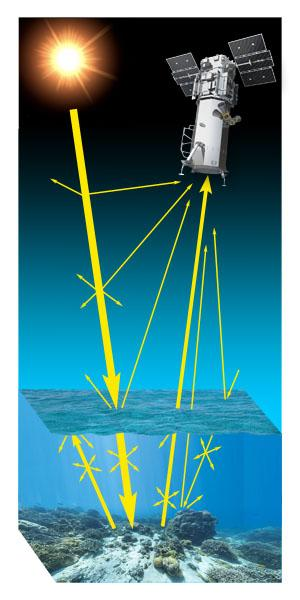
\includegraphics[width=\textwidth]{CBYK292WkAAIkzH.jpg}
    \caption{Graphic demonstrating Satellite Derived Bathymetry}
    \label{fig:sdb}
\end{figure}

\par
The limitations of the \ac{SDB} method are based on water depth and clarity.
As depth increases light is unable to pass through the water column to the bottom.
The depth that light can penetrate is determined by the characteristics of the water.
Clear water will allow for much deeper depths to be predicted, where as murky, cluttered water limits the maximum depth.
Environmental characteristics such as sediment composition and weather affect the clarity of water \cite{vinayaraj2016satellite}.

\par
Current \ac{SDB} models can predict bathymetry with a \ac{RMSE} of less that 2.5 meters at a maximum depth of 50 meters.
Work performed by \cite{vinayaraj2016satellite} has improved the depth by using blue light sensing techniques.
Work performed by \cite{chybicki2018three} improved the accuracy by using advanced regression models when measuring the wavelengths.
\ac{SDB} models are ideal for coastal areas with a high water visibility.

\subsection{Aggregated Earth Gravitational Models (EGM)}
Work performed by Smith and Sandwell \cite{smith1994bathymetric}\cite{smith1997global} pioneered the use of Earth Gravitational Models (EGM).
They proposed that the relationship between seafloor topography and sea surface gravity is conveniently related \cite{smith1994bathymetric}.
Their work identified the wavelength bands at which this relation holds true.
They identified the areas that could be predicted with this relationship and used sparse ship soundings to fill in gaps of their predictions.
Areas with large seamounts found the correlation to be strongest, while areas of flat sediments found the correlation to be weakest.
They named this technique the "Inverse Nettleton Procedure" and used a simple linear regression model to exploit this correlation and improve existing aggregated datasets.

\begin{equation}
    b(x) = D(x) + s(x)g(x) \label{eq:egm}
\end{equation}

\par
Smith and Sandwell aggregated their predicted values from their \ac{EGM} with ship based Multi Beam Echo Sounding sonar data.
The sonar data is sparse, but provides accurate readings of the ocean's bathymetry.
This aggregation yielded global coverage up to 81 degrees latitude.
The aggregation yielded prediction accuracy within ~100 meters in coastal waters, and ~200 meters in the global ocean space.

%Discuss the STRM Global Dataset here in detail....
\par 
This work was later improved in \cite{becker2009global}.
The model was substantially improved by increasing the number of ship soundings and increasing the aggregation sources.
Ten external datasets were aggregated for the SRTM30 grid.
Agencies in these sources include \ac{NAVO}, \ac{GEBCO}, \ac{NOAA}, \ac{NGA}, and \ac{JAMSTEC}.
These datasets include high resolution coastal bathymetry from around the world and greatly increased the global accuracy.

%Spelling check big time bruh
\par
The limitations of aggregated \ac{EGM}s is based on correlation uncertainty and unknown ocean features.
Sediment density drives the correlation between sea surface gravity and bathymetry.
A dense geoid will generate greater sea surface gravity than a less dense geoid.
Flat sea floors with a less dense composition can appear lower than normal.
This is all controlled by the scaling factor described in \cite{smith1994bathymetric} and shown in equation \ref{eq:egm}. 
However, there is not a optimal scaling factor for the entire world.
Identifying an optimal scaling factor for an area will require knowledge of the sediment type in the global scale.


\subsection{Machine Learning Optimized \ac{EGM}}
The aggregated \ac{EGM} is a physics based model that wants the relationship between gravity and bathymetry to be directly correlated.
This correlation is often non-trivial to define due to environmental factors.
The nondeterministic behavior is compensated by the scaling factor mentioned in the previous section.
Attempts to optimize this scaling factor have been made, and \ac{ML} has shown much promise in this regard.

\par
The work preformed by \cite{jena2012prediction} used \ac{ML} to optimize their gravitational regression models.
Instead of identifying an optimal scaling factor deterministically, they used an \ac{ANN} to optimize the scaling factor.
This was done using precise \ac{MBES} data as truth data and satellite altimeter data.
This method was tested on a localized swatch of ocean in the Arabian Sea.

\par
This optimization improved upon the current physics models.
Their model could predict bathymetry within a \ac{RMSE} of ~129 meters for flat sea floor.
Geoids resulted in a \ac{RMSE} of ~179 meters.
Both of these results are globally similar with aggregated models, while boasting increased accuracy in their localized training area of the Arabian Sea.

%\subsection{Machine Learning Models}
    \section{Data Analysis}
\setlength{\parindent}{10ex}

All data used in this work was aggregated from existing studies.
The ETOPO dataset was used for bathymetry soundings \cite{national1988etopo}.
All other features and their origin datasets can be seen in the table below. %Insert point to figure yadaydada

%This section is for defining the data being used in the experiment
%It should define where the data came from and its format
%I can also explain any of the special stuff I am doing (Binning for example)
%

\begin{center}
    \begin{table}[htb]
        \begin{tabular}{ |p{0.5\textwidth} p{0.5\textwidth}| }
            \hline
                \textbf{Feature} & \textbf{Origin Study} \\
                \hline
                Mantle Density & CRUST1 \cite{laske2013update} \\
                LAND One Hot & ETOPO \cite{national1988etopo} \\
                Crust Thickness & CRUST1 \cite{laske2013update} \\
                Low, Mid, High Crust Density & CRUST1 \cite{laske2013update} \\
                Estimated Current East, North, Mag & HYCOM \cite{chassignet2009us} \\
                Sea Nitrate, Phosphate, Salinity Measurements & NASA Studies \cite{meissner2018salinity} \cite{parekh2005decoupling}  \\
                Sea Temperature, Silicate Measurements & NASA Studies \\
                Sediment Thickness & CRUST1 \cite{laske2013update} \\
                BioMass Features & \cite{wei2010global} \\
                Geoid Features & EGM \cite{pavlis2008earth} \\
                Wave height, period & WAVEWATCH \cite{tolman20072007} \\
            \hline
        \end{tabular}
        \label{table:FEATURE_LIST}
        \caption{List of Ocean Features used in Models for this Project.}
    \end{table}
\end{center}
%I am using this section to introduce the feature selection method that I preformed
%Maybe I can flesh this out more and talk about it in def??
%Maybe make a diagram for the flow of the GA?
\subsection{Feature Selection}
Feature selection was used to identify the most relevant features for classification.
This important step in the \ac{ML} pipeline removes noise from irrelevant data.
This work used a genetic algorithm approach for feature selection \cite{yang1998feature}.
Other approaches that were considered included a grid search, dimensional analysis, and simple variable correlations.
These approaches were found to either take to long, or simply not offer enough improvement to the model.
Where as, the genetic algorithm approach gave relatively quick model improvements with little effort.
See \ref{fig:GA} for an illustration of a generic genetic algorithm.

\par
Using a genetic algorithm for feature selection is a simple application of the original process.
The initialized population is a set of random binary strings.
Each string has a character length equal to the number of features in our feature space.
The binary characters represent if a feature is active or inactive.
Essentially these strings represent a set of features to use in training a model.
The fitness of that string is represented by the resulting models accuracy.
Selection is preformed by choosing the most accurate models, and their characteristics are passed to the next generation.
A simple crossover mutation of the strings is used, along with a modest 5 percent mutation rate.
Upon termination the resulting fittest string is used as the selected features.


\begin{center}
    \begin{figure}[h]
        \caption{Diagram of Generic Genetic Algorithm}
        \label{fig:GA}
        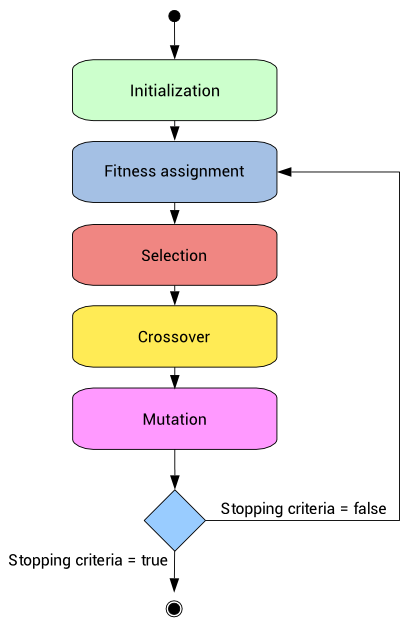
\includegraphics{genetic_algorithm.png}
    \end{figure}
\end{center}

%This decribes how the grid files are used and oragnized...
%They are essentially binary files...
\subsection{Data Representation}
Representing global data is typically done using a grid.
Where each grid represents a coverage of the Earth's surface.
This representation can an average of the data across the coverage of that cell, but is not guaranteed.
The data used in this work has been organized into a grid for this purpose.
Each grid represents a cell centered data point, and they are organized into a EPSG:3857 \ac{CRS}.

\par
The spatial resolution of a grid defines its coverage.
This spatial resolution can be described as the height and width of a grid.
This height and width is not physically constant.
For example, a cell at the equator is larger and covers more physical area than a cell at the poles.
However, this is the best way to represent the data in a consistent and structured manner.

\par
All data in this project has been organized into two minute bathymetry grids.
A two minute bathymetry grid has a spatial resolution of 0.034 degrees per cell.
This is approximately 3 kilometers of spatial coverage.
The grids have a column length of 5400 and a row width of 10800.

\par
This resolution was chosen for experiments to conserve memory and time.
Larger grids have a exponentially larger memory and computational footprint.
I used the \ac{ETOPO}2v2 \cite{national1988etopo} dataset as the source of the two minute bathymetry grid.
Finer resolution datasets exist, such as the SRMT30 \cite{becker2009global} at 30 second resolution.
However, portions of data in that set is up sampled from lower resolution datasets such as ETOPO.
In any event, the two minute resolution offered a good balance of memory, accuracy, and computational costs.

\subsection{Ocean Features}
Similar to bathymetry values, all extracted ocean features for this project were organized into a two minute bathymetry grid.
They were aggregated from several projects.
Absent data points was either interpolated, or filled with default values.
See \ref{table:FEATURE_LIST} for a complete list of all features.

\par
\ref{fig:bathyxfish} shows the relationship between estimated fish biomass and bathymetry.
There is a direct relationship that trends toward less biomass as the ocean gets deeper.
Naturally, this relationship is explained by the availability of food and light at such lower depths.
\ref{fig:bathyxfauna} shows a similar relationship to the fish biomass.

\par
\ref{fig:bathyxdensity} shows a example of a inverse relationship to bathymetry.
\ref{fig:pairplot} Shows a pair plot of all the features used in training.
The diagonal in the pair plot will show the correlation of point distributions in each individual plot.
Each of the discussed plots were taken from data in the south Pacific ocean.
This was done as a isolated demonstration of the data.
%Talk about the plots here and include them once seaborn has decided to stop being dumb...

\begin{figure}[h]
    \centering
    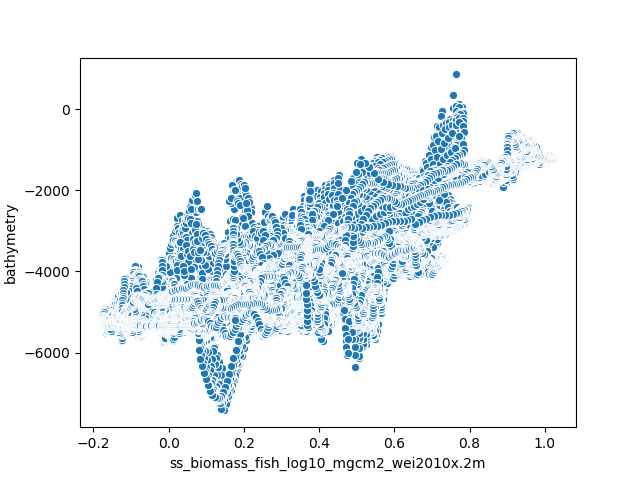
\includegraphics{Bathymetry_X_SS_BIOMASS_FISH_LOG10_MGCM2_Wei2010x.png}
    \caption{Graph of Bathymetry and Estimated Fish BIOMASS}
    \label{fig:bathyxfish}
\end{figure}

\begin{figure}[h]
    \centering
    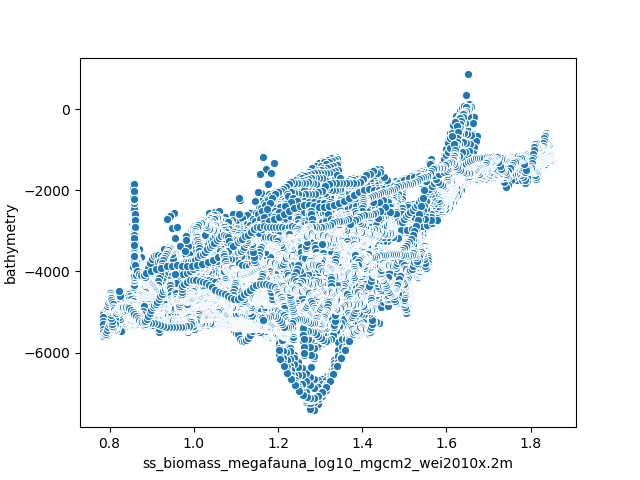
\includegraphics{Bathymetry_X_SS_BIOMASS_MEGAFAUNA_LOG10_MGCM2_Wei2010x.png}
    \caption{Graph of Bathymetry and Estimated MegaFauna Bio Mass}
    \label{fig:bathyxfauna}
\end{figure}

\begin{figure}[h]
    \centering
    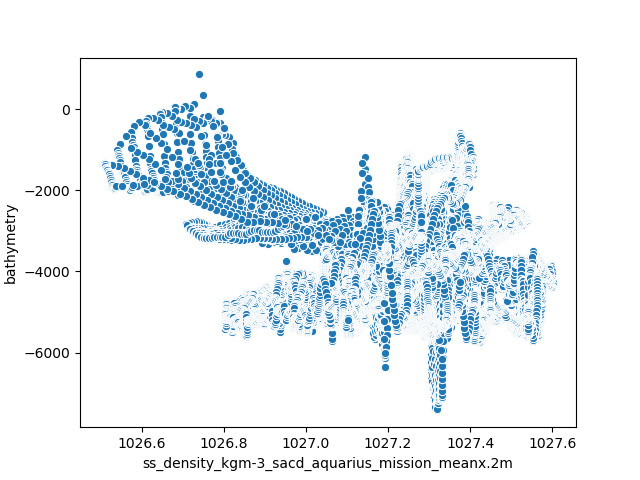
\includegraphics{Bathymetry_X_SS_DENSITY_KGM-3_SACD_Aquarius_MISSION_MEANx.png}
    \caption{Graph of Bathymetry and Estimated Crust Density}
    \label{fig:bathyxdensity}
\end{figure}

\begin{figure}[h]
    \centering
    \includegraphics{pairplot.png}
    \caption{Pair Plot of All Features Used in Training}
    \label{fig:pairplot}
\end{figure}

%Maybe I can talk about some of the correlations I preformed here???? A few graphs perhaps???
%Maybe talk about the PCC???
%Possibly need to talk about the breadth of features here....

\subsection{Bathymetry Values}
ETOPO2v2 is used for the bathymetry soundings \cite{national20062}.
This extension of the ETOPO2 dataset \cite{national1988etopo} is a more accurate and updated version of the ETOPO2 dataset.
Specifically this version eliminates a westward bias present in the original version.
The two minute \ac{ETOPO} dataset was used to match the chosen resolution for this work.
\ac{ETOPO} was aggregated by the \ac{NGDC} which is a department of \ac{NOAA}.

\par
Land topography is included in the \ac{ETOPO} dataset.
A mask was created to mask out the land topography in all training datasets.
The masking is the LAND One hots feature listed in \ref{table:FEATURE_LIST}.
This is applied to the data before training.

%There is a better was to describe why the features were binned like this
%I want to describe the value that was added by binning my data into classes!
\par
The classification preformed in this work used binned bathymetry from \ac{ETOPO}.
These classes were partitioned on a interval of 150 meters.
This partitioning scheme was chosen to improve upon the results from a similar project \cite{jena2012prediction}.
The binning is preformed to leverage the unique advantages inherent to classification problems and test if this problem is better suited for classification.
For example, the use of metrics such as a confusion matrix makes comparing the performance of the model significantly easier.

    \section{Results}
\setlength{\parindent}{10ex}

This section contains the results for the experiments performed by this work.
Including results for the regression, classification, and novel grid optimized model.
Each section includes figures representing the metric scores.

\subsection{Regression Results}
Regression \ac{ML} models were fit in order to compare to existing physics models.
Three models were fit to the data: 
an SVM regression model, a Naive Bayes regression model, and a simple linear regression model.
These models were trained against a reduced set of data shown in figure \ref{fig:trainset}, and validated against the rest of the world.
Each model was fit against selected features from the Genetic Algorithm feature selector.
The \(R^2\) score for each model can be found in figure \ref{fig:r2_barplot_regression}.
The RMSE of each model can be found in figure \ref{fig:rmse_barplot_regression}.



\begin{figure}[h]
    \centering
    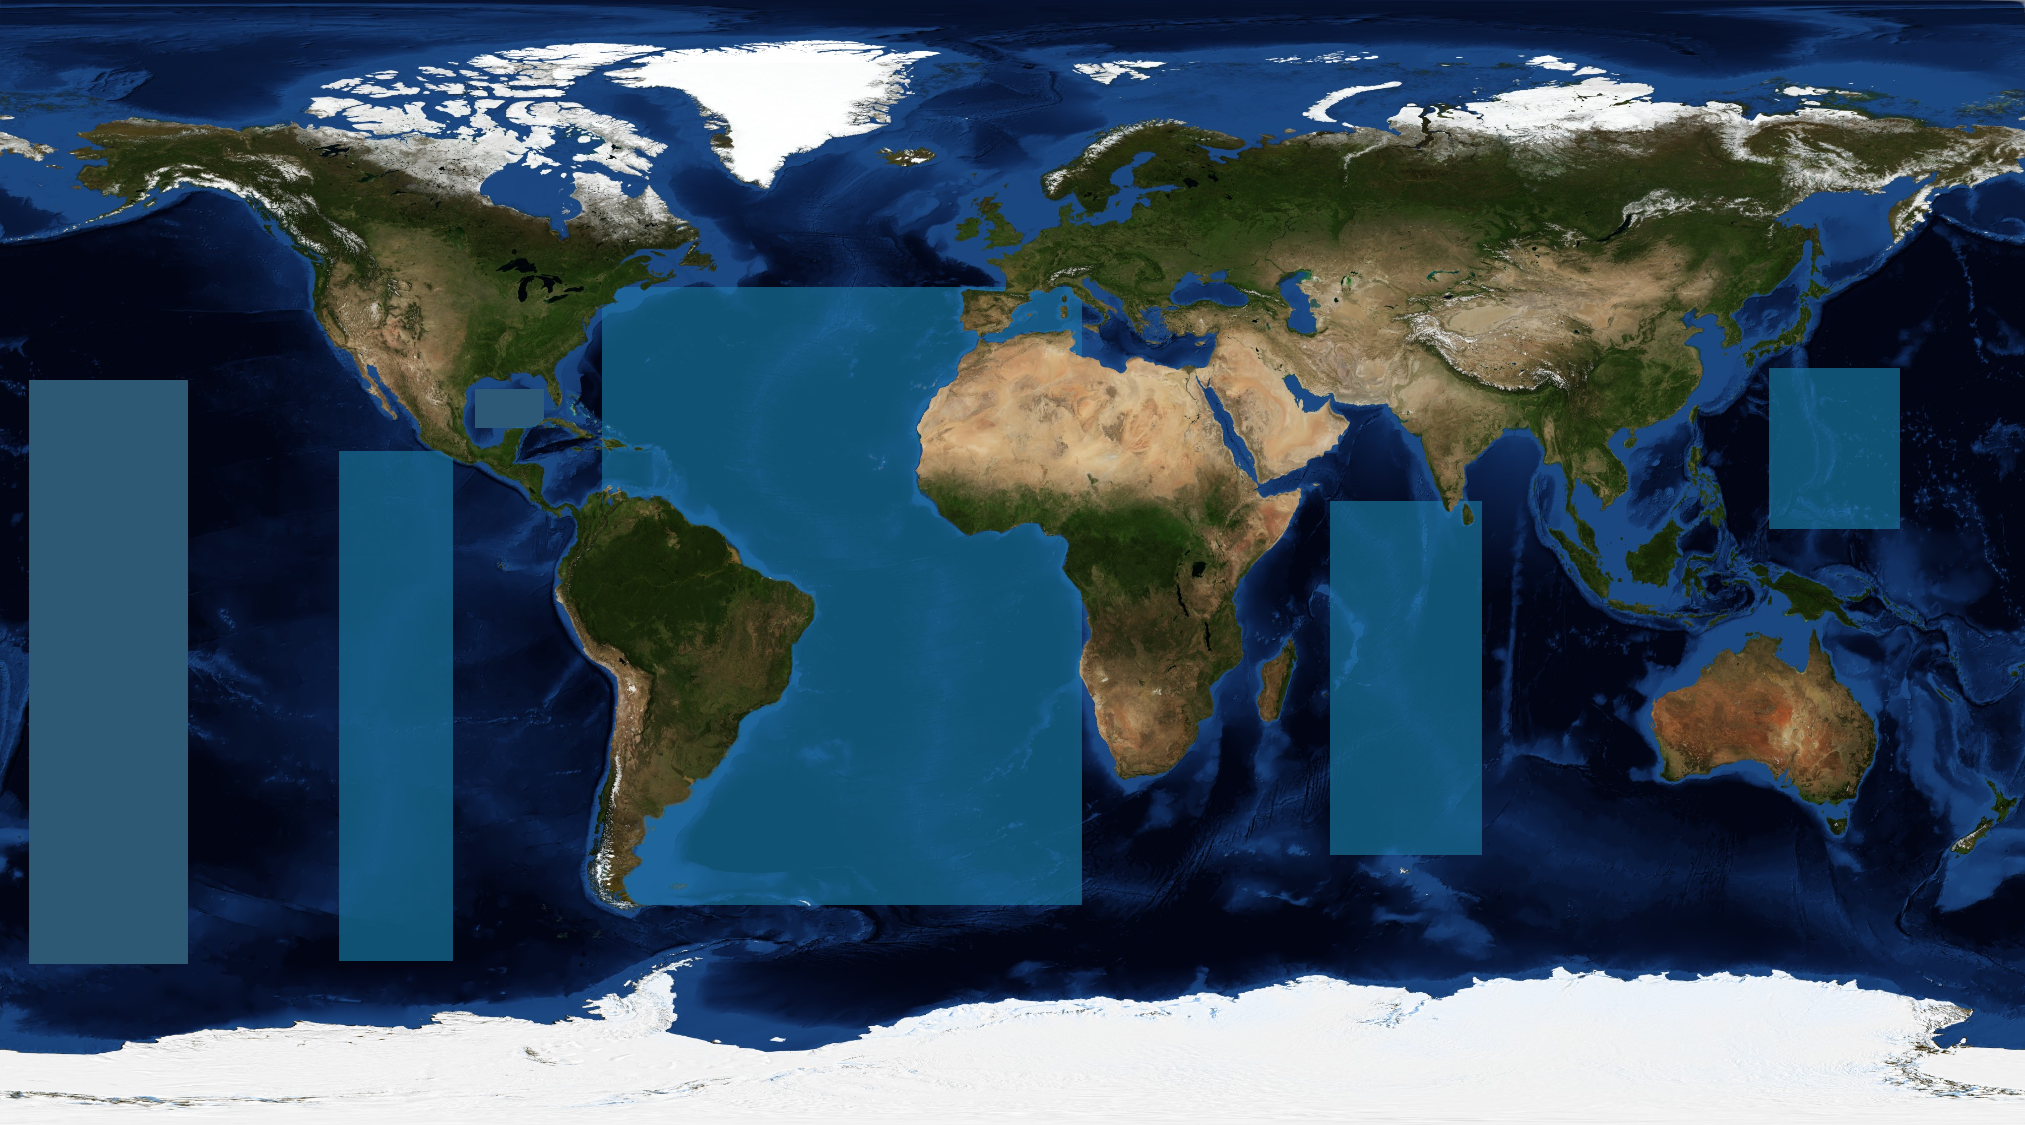
\includegraphics[width=\textwidth]{worldtraininglocal.png}
    \caption{Figure demonstrating initial training sets.}
    \label{fig:trainset}
\end{figure}

% \begin{table}[htb]
%     \centering
%     \begin{tabular}{|c c c|}
%         \hline
% 		\textbf{Model} & \textbf{\(R^2\)} & \textbf{RMSE} \\
% 		\hline
% 		SVM Regression & 0.841 & 365.23m \\
% 		Naive Bayes & 0.884 & 294.92m \\
%         Linear Regression & 0.885 & 265.43m \\
% 	    \hline
%     \end{tabular}
%     \label{table:REGRESSION_RESULTS}
%     \caption{Regression Results}
% \end{table}

\begin{figure}[h]
    \centering
    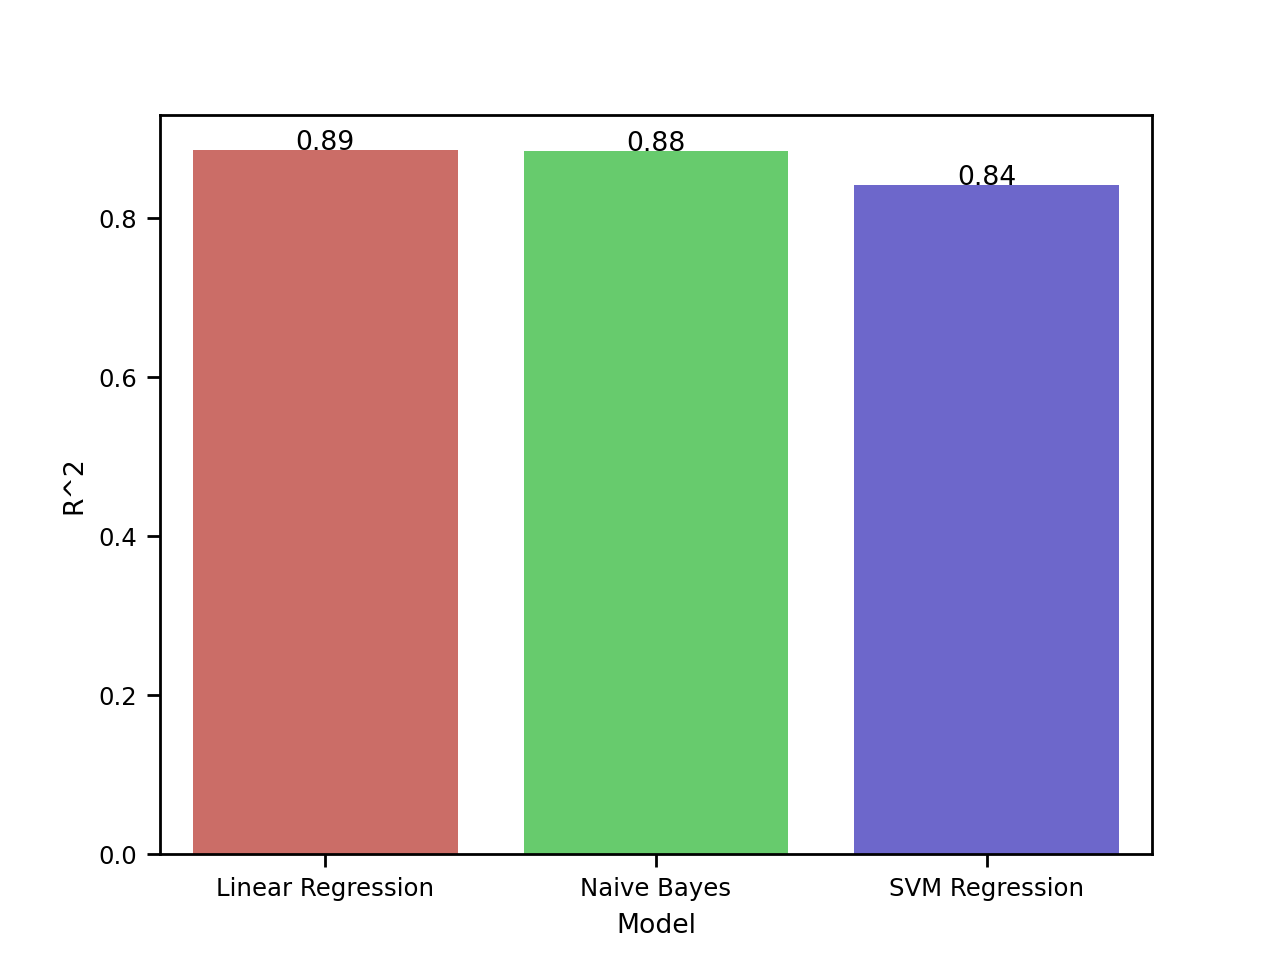
\includegraphics[width=\textwidth]{rsquared_barplot_regression.png}
    \caption{Bar chart showing \(R^2\) score for each model}
    \label{fig:r2_barplot_regression}
\end{figure}

\begin{figure}[h]
    \centering
    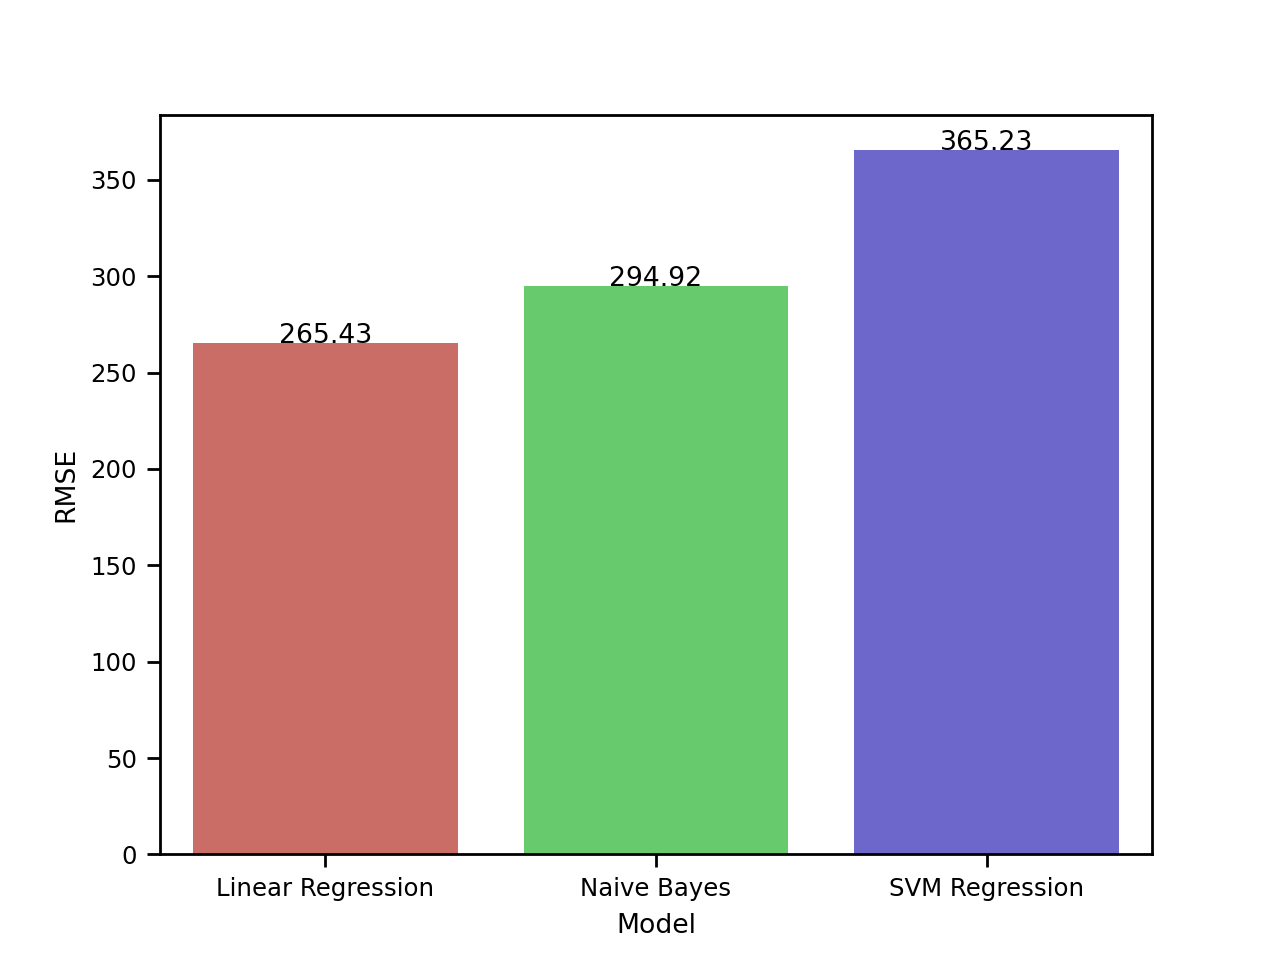
\includegraphics[width=\textwidth]{rmse_bar_regression.png} 
    \caption{Bar chart showing RMSE for each model}
    \label{fig:rmse_barplot_regression}
\end{figure}

% \subsubsection{Regression Results Discussion}
% \cite{jena2012prediction} achieved a \ac{RMSE} of \~{}175m in their optimized model.
% The linear regression model I fit is 100 meters less accurate than the optimized model used in \cite{jena2012prediction}.
% However, the purpose of the test is not to achieve accurate predictions, but to identify if \ac{ML} models can be viable.
% Therefore, the accuracy of these models is less important than identifying the viability of the models.
% The training data used is essentially predicted bathymetry, but shows that fitting a model to true bathymetry will yield a similar result.
% Analyizing the \(R^2\) score gives evidence of the viability of the model.
% This score suggests that there are underlying relationships in the model that can be used to train a successful model.

\subsection{Classification Results}
\setlength{\parindent}{10ex}
%Maybe reword this opening chapter???
To facilitate classification, trained models need to predict discrete values instead of continuous values.
This conversion was executed by mapping the bathymetry values into discrete classes.
This conversion proved to be trivial because of the ordered nature of bathymetry.
Classification models are simpler and easier to fit than regression models.
Ideally, the decision surfaces will benefit from the conversion and yield better results.
This makes it difficult to compare directly to the error reported in existing physics models.
A set of metrics including: precision, recall, f1 score, and balanced accuracy were used to analyze the viability of the models.

\par
The ordinal classes were binned on a interval of 150 meters.
This was done to easily compare accuracy to model in \cite{jena2012prediction}.
Validation was preformed using a 10 fold cross validation using balanced accuracy as the scoring function.
The F1 results for each model can be found in figure \ref{fig:f1_barplot_classification}.
The Balanced Accuracy for each model can be found in figure \ref{fig:balacc_barplot_classification}

\par
The Decision Tree classifier performed significantly worse than the other models.
The 47\% balanced accuracy is not usable for predictions.
Potentially, parameter tuning, and maybe feature selection could improve this model.

% \begin{table}[htb]
%     \centering
%     \begin{tabular}{|c c c|}
%         \hline
% 		\textbf{Model} & \textbf{Average F1 Score} & \textbf{Mean Balanced Accuracy} \\
% 		\hline
% 		Random Forest & 0.81 & 0.82 \\
%         Bagging & 0.80 & 0.79 \\
%         Decision Tree & 0.44 & 0.47 \\
%         \hline
%     \end{tabular}
%     \label{table:CLASSIFICATION_RESULTS}
%     \caption{Classification Results}
% \end{table}

\begin{figure}[h]
    \centering
    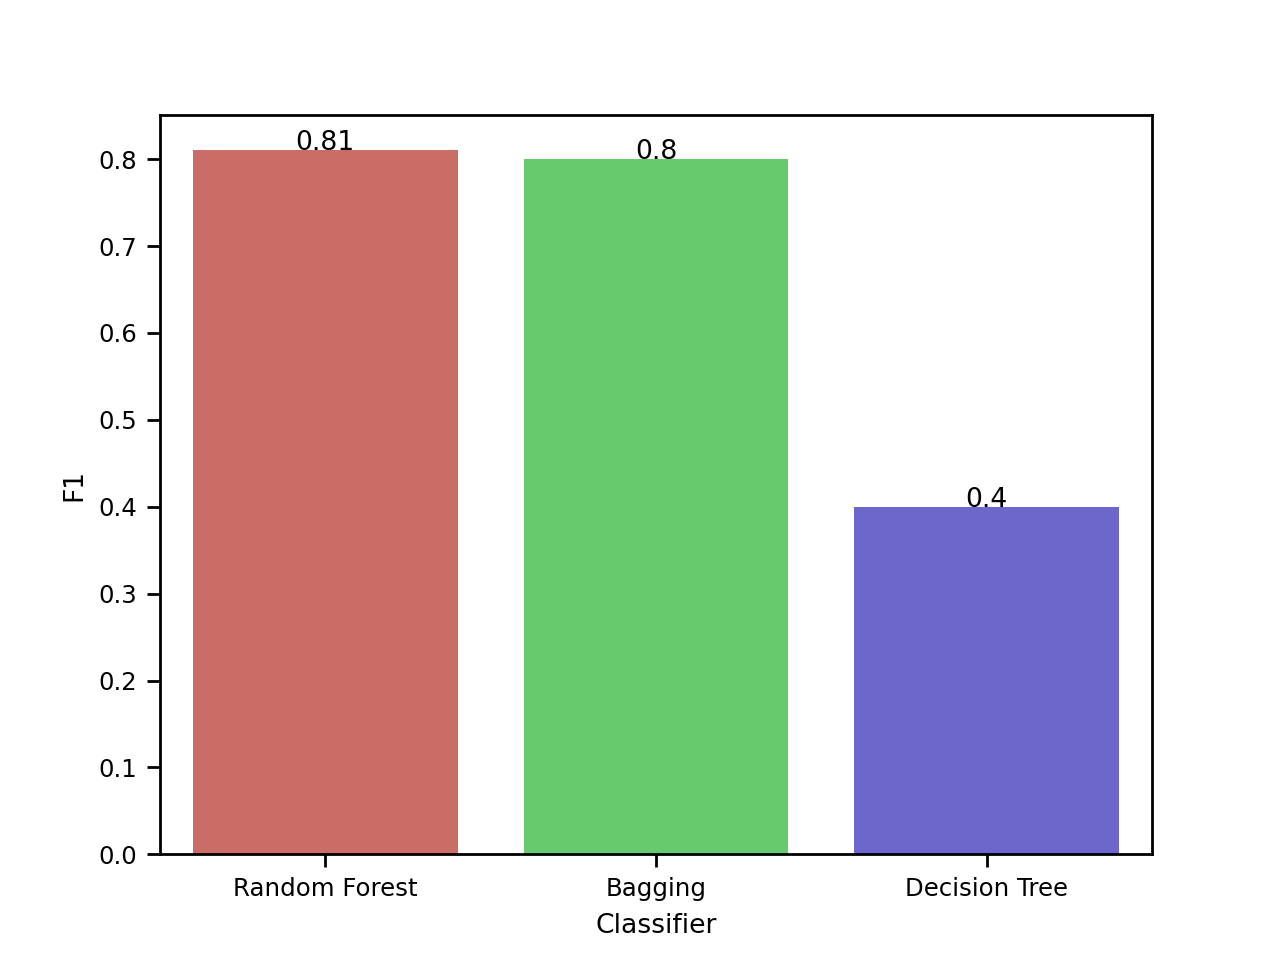
\includegraphics[width=\textwidth]{f1_bar_classification.png}
    \caption{Bar chart showing F1 score for each classifier}
    \label{fig:f1_barplot_classification}
\end{figure}

\begin{figure}[h]
    \centering
    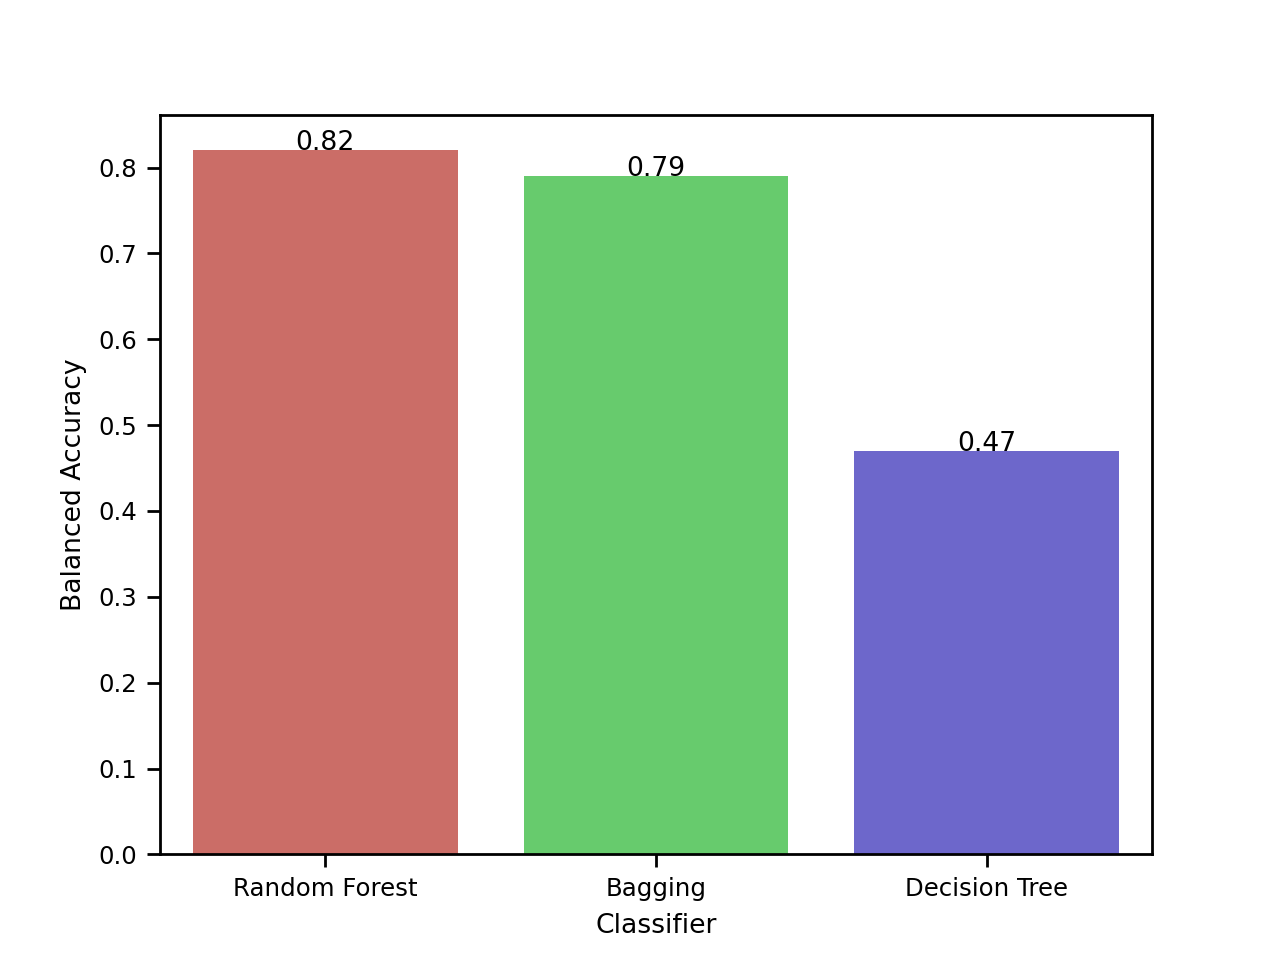
\includegraphics[width=\textwidth]{balacc_bar_classification.png}
    \caption{Bar chart showing balanced accuracy for each classifier}
    \label{fig:balacc_barplot_classification}
\end{figure}

\subsection{Optimized Grid Model}
\setlength{\parindent}{10ex}
%Purpose of this section is to identify the optimized grid structure.
%I need to check with Hoque to identify what I should and shouldnt include
%I need to consider rewording this and restructuring to manage the correctness for example etc.
% Further analysis of figure \ref{fig:rfc_report} shows that models are sensitive to potentially local characteristics.
% In an attempt to test this notion and increase the accuracy of these models a novel model selection method was employed.
% The objective being to identify if a model will predict more accuractly based on geospatial location.
% The hypothysis being that decision boundaries across different models will respond to features based on location.

The Grid Optimized Model Injector Classifier is concerned with testing the best model fit hypothesis.
The theory being that there is not a best fit model for predicting bathymetry across the Earth.
For example, a model may be excellent at predicting shallow bathymetry where there is a particular feature that is sensitive to a sediment type.
Where as, another model may be excellent at predicting bathymetry in deep water scenarios.
This novel Grid Optimized Model Injector tests this theory by implementing a model that optimizes by geospatial location.

\begin{figure}[h]
    \centering
    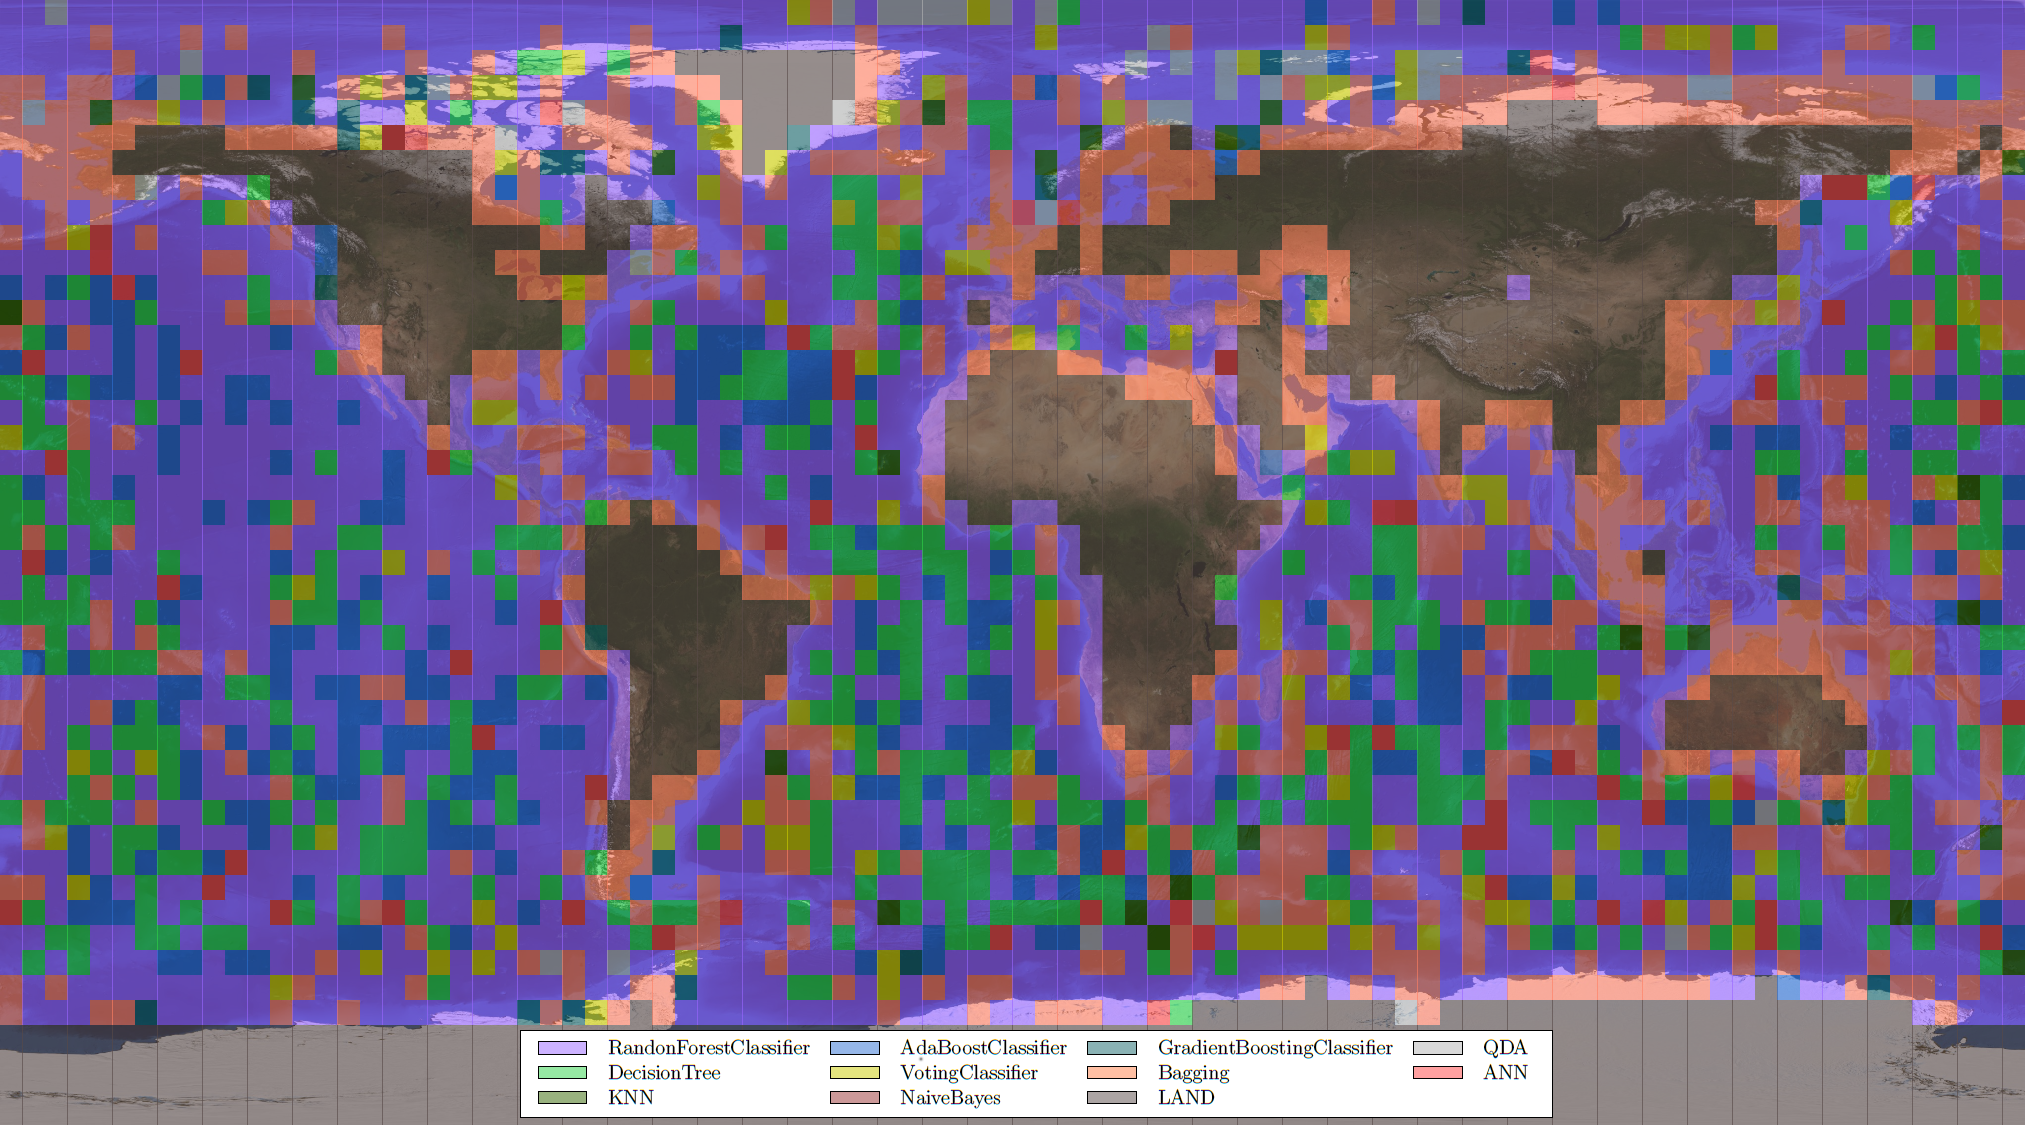
\includegraphics[width=\textwidth]{optgriddraft.png}
    \caption{Graphic Showing the World Coverages and Successful Models}
    \label{fig:coveragegrid}
\end{figure}

%Give the background for the idea in this section!
\subsection{Analysis of Global Model Optimization}
This hypothesis was tested by building a model that optimizes by geospatial location.
In order to optimize by location a cache of "best fit" models per location needed to be created.
This can be performed by comparing the performance of a set of models for predicting every point in a grid.
However, this can take an extremely long time because of the size of these geospatial grids.
To simplify this experiment, for fake of time and computing resources, the world was instead split into N coverages.
These coverages represent an area of the Earth and will suffice for the experiment of comparing model performance across geospatial locations.
The performance of a set of models for each coverage was recorded.
The best performing model in that coverage was then exported and saved to a map of best fit models to a geospatial bounding box.
The results of this experiment are displayed in figure \ref{fig:coveragegrid}.

\begin{figure}[h]
    \centering
    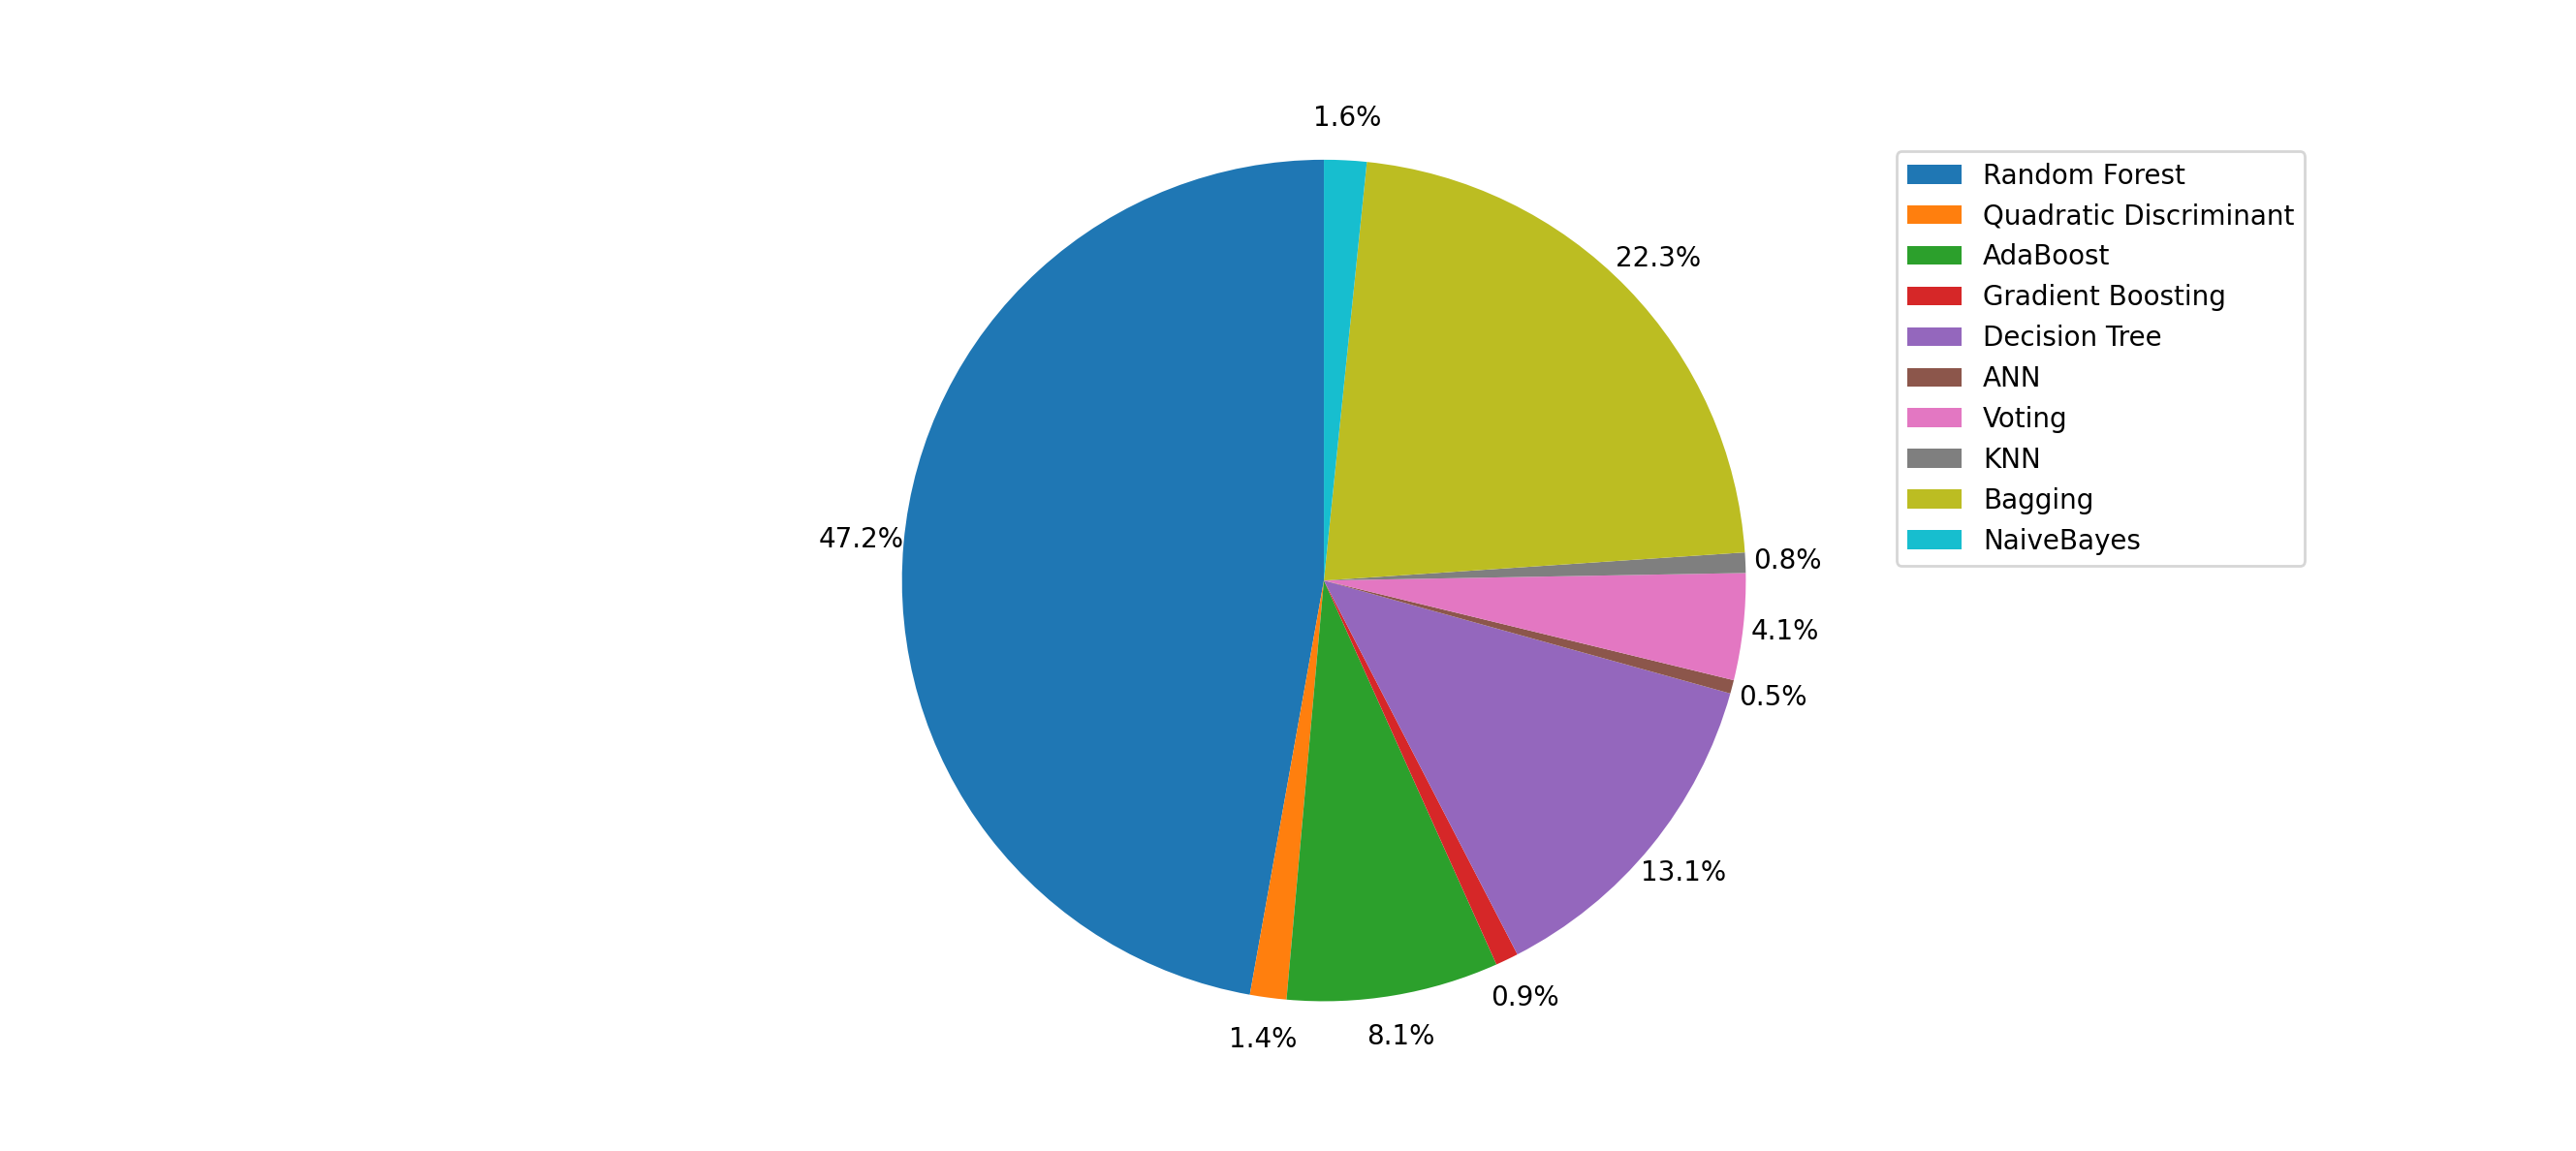
\includegraphics[width=\textwidth]{best_fit_percentage.png}
    \caption{Pie plot showing the percentage of coverages where a model was "best fit"}
    \label{fig:pie_best_fit}
\end{figure}

\par
Figure \ref{fig:coveragegrid} shows several interesting things.
Figure \ref{fig:pie_best_fit} shows the percentage that each model was a best fit.
The random forest classifier was the best fit model for a large portion of the oceans.
On the other hand, the Bagging classifier consistently performed well along the coast lines.
The reasons for why these classifiers may have performed so well in those areas will be touched upon in the discussions section.


\begin{figure}[h]
    \centering
    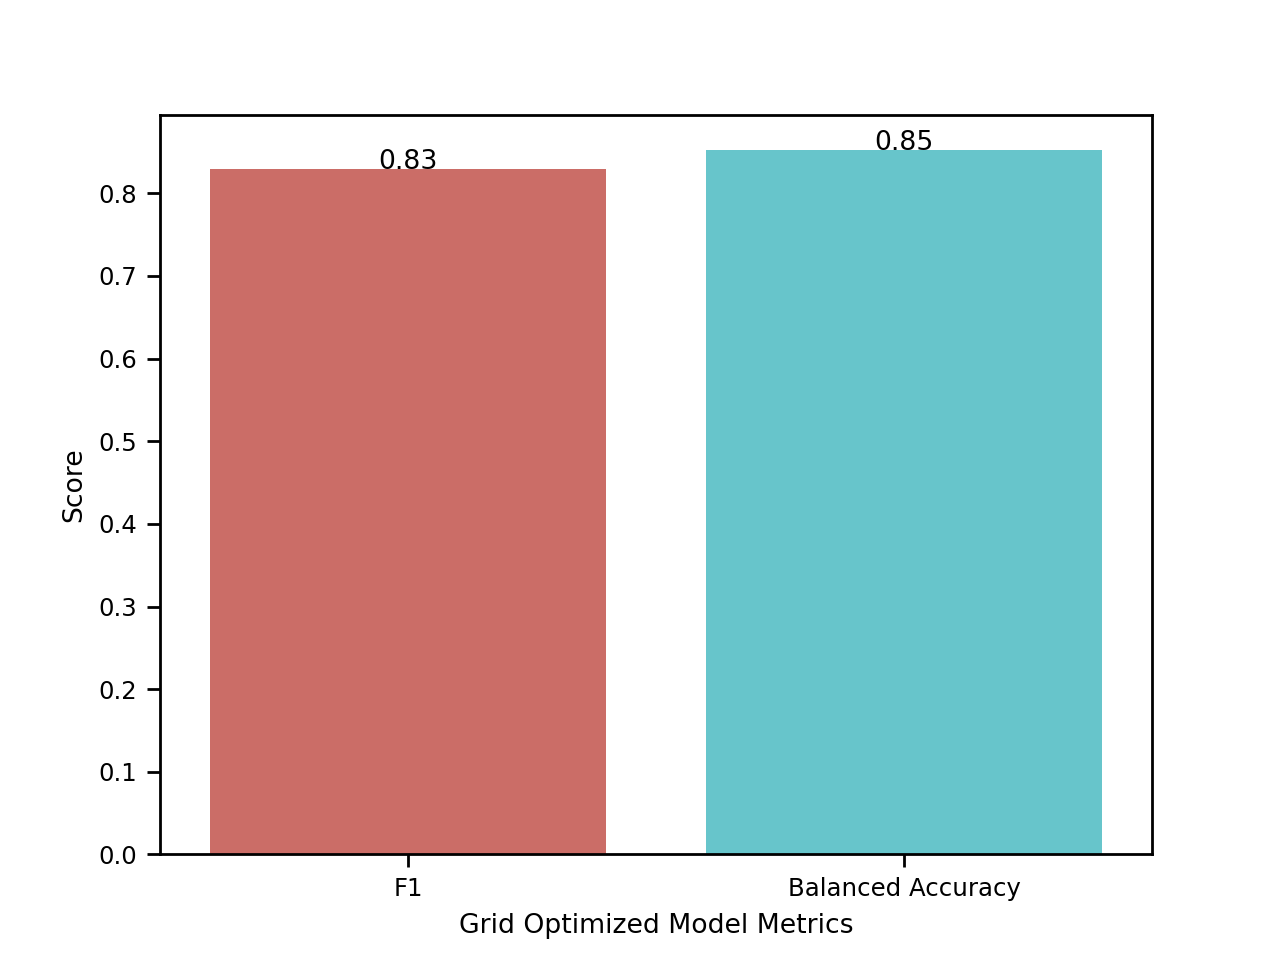
\includegraphics[width=\textwidth]{grid_opt_results.png}
    \caption{Bar chart showing Grid Optimized Model results}
    \label{fig:grid_opt_barplot}
\end{figure}
%In this section I am defining what the Grid optimization is and why it matters.
%There may be a better name for this?? Who knows really...
\subsubsection{Grid Optimizing Results}
Using the successful model for each coverage as a \textit{optimum} selection.
The optimum selection improved the prediction accuracy of the model by several percent.
See figure \ref{fig:grid_opt_barplot} for the results of the model.



    \section{Results Discussion}
\label{sec:discussion}
\setlength{\parindent}{10ex}
This chapter explores the interesting concepts and emergent ideas that stem from this work.
It is divided into a discussion of the three core experiments performed, specifically, the regression, classification, and novel grid optimization experiments.

\subsection{Regression Results Discussion}
\cite{jena2012prediction} achieved an \ac{RMSE} of \~175m in their optimized model.
Their model used \ac{ML} to predict an optimum scaling factor \textbf{S}.
The linear regression model fit in this project is 100 meters less accurate than the optimized model used in \cite{jena2012prediction}.
The purpose of the test is not to achieve accurate predictions, but to identify if \ac{ML} models can be viable for predicting bathymetry.
Therefore, the accuracy of these models is less important than identifying the viability of the models.
The training data used is predicted bathymetry, but shows that fitting a model to true bathymetry will yield a similar result.

\subsection{Classification Results Discussion}
The Random Forest model excelled with a balanced accuracy of 82\%.
Breaking down the results by class, the classifier predicted some classes with greater precision than others.
This indicates that the decision boundary responded to certain trends in the data.
In general, the Random Forest classifier performed better overall, which is why it was the best performing classifier for 47.2\% of the world.
This percentage can be seen in Figure~\ref{fig:pie_best_fit}.

\par
The Bagging classifier performed on par with the Random Forest Classifier with a balanced accuracy of 79\%.
However, Figure~\ref{fig:coveragegrid} shows that the bagging classifier performed best around coastlines.
This suggests that the model responds well to shallow waters.
Shoreline data will also be consistently more accurate because of the proximity to land.
Most of the world's high-resolution bathymetry is shoreline, and it is possible that the model responded to the quality data.


\par
The classification results show that labeling bathymetry can improve the performance of the models.
In this work, it was tested that a random forest classifier can predict 82\% of the world's predicted bathymetry within 150 meters of accuracy. 
However, what is more interesting to analyze is the behavior of the models.
The data used in training comes from aggregated external datasets and a predicted bathymetry dataset.
The predictions of these models are being compared to predicted bathymetry which represents the accuracy with relation to predicted values.
This means that the accuracy in these models is not indicative of truly predicting global bathymetry.
It does show that an \ac{ML} model can be fit to data and be used to predict bathymetry, and if actually measured bathymetry and ocean features were used in training, the results would be comparable.
Furthermore, parameter tuning, model selection, and dynamic feature selection could be used the increase the accuracy beyond current results.

\par
Interestingly, some models excel along fault lines.
For example, the decision tree classifier in Figure~\ref{fig:coveragegrid} performs well along what appear to be fault lines.
However, when making predictions in the global scope the classifier is very inaccurate.
This suggests that a classifier can be optimized using geospatial position.



\subsection{Grid-Optimized Model Discussion}
%The world wide ETOPO bathymetry dataset \cite{national1988etopo} at two minute resolution is used for valadation and metrics.
%This dataset is treated as the ground truth for all predictions.
%During the experiment, a one third holdout was used for validation in some cases.
%For finding the optimum model for a coverage a 10 fold cross validation was utilized.

%Include metrics information here.... possibly graphs and a list of scores? I dont really know.

%I dont like how I worded this whole section...
%The idea here is that I want to say "Hey, these people did this research and found the their regression model preforms poorly for predicting seamounts espicially after 500m.
%I clearly noticed a similar trend, but saw better preformance from some models than others. 
%This research is to identify those coverages and then use those results to build a super classifier.
%These metrics are important for identifying where the models preform well. 
\par
The Grid Optimized Model Injector improved the accuracy of predictions by \~{}5\%.
These results are displayed in Figure~\ref{fig:grid_opt_graph}.
Obviously, the model selection and subsequent injection improved the results of this classifier, creating an ensemble of many models and selecting them on demand.
This could be caused by geophysical characteristics that benefit one classifier.
For example, in Figure~\ref{fig:coveragegrid} the Decision Tree classifier performed best along what appears to be fault lines.
It is possible that the characteristics related to being in proximity to a fault line benefited the model's decision boundary. 

\par
Clearly, Figure~\ref{fig:coveragegrid} provides evidence that model decision boundaries are sensitive to the features based on location.
This leads to the theory that there is not a single best fit model for predicting global bathymetry.
Analysis of Figure~\ref{fig:coveragegrid} shows interesting consistencies that raise questions about the underlying features.
For example, in Figure~\ref{fig:coveragegrid} the Bagging classifier appears to perform best around coast lines.
This is consistent for most of the globe.
However, in some coastal areas the Random Forest Classifier performs best. 
It is possible these areas are linked to port cities and the high-resolution bathymetry collected from shipping lanes.

\par
Another interesting consistency is around fault lines.
The coverages where the DecisionTree classifier performed best seems to follow fault lines.
It is possible there is a geospatial attribute that contributes to this success, or a specific feature in these locations that contributes to the DecisionTree classifier's performance.
The AdaBoostClassifier also performs well around fault lines, but to a lesser extent.
It is possible there are trends in the data that explain why the AdaBoostClassifier shows this behavior.

\begin{figure}[htp]
    \centering
    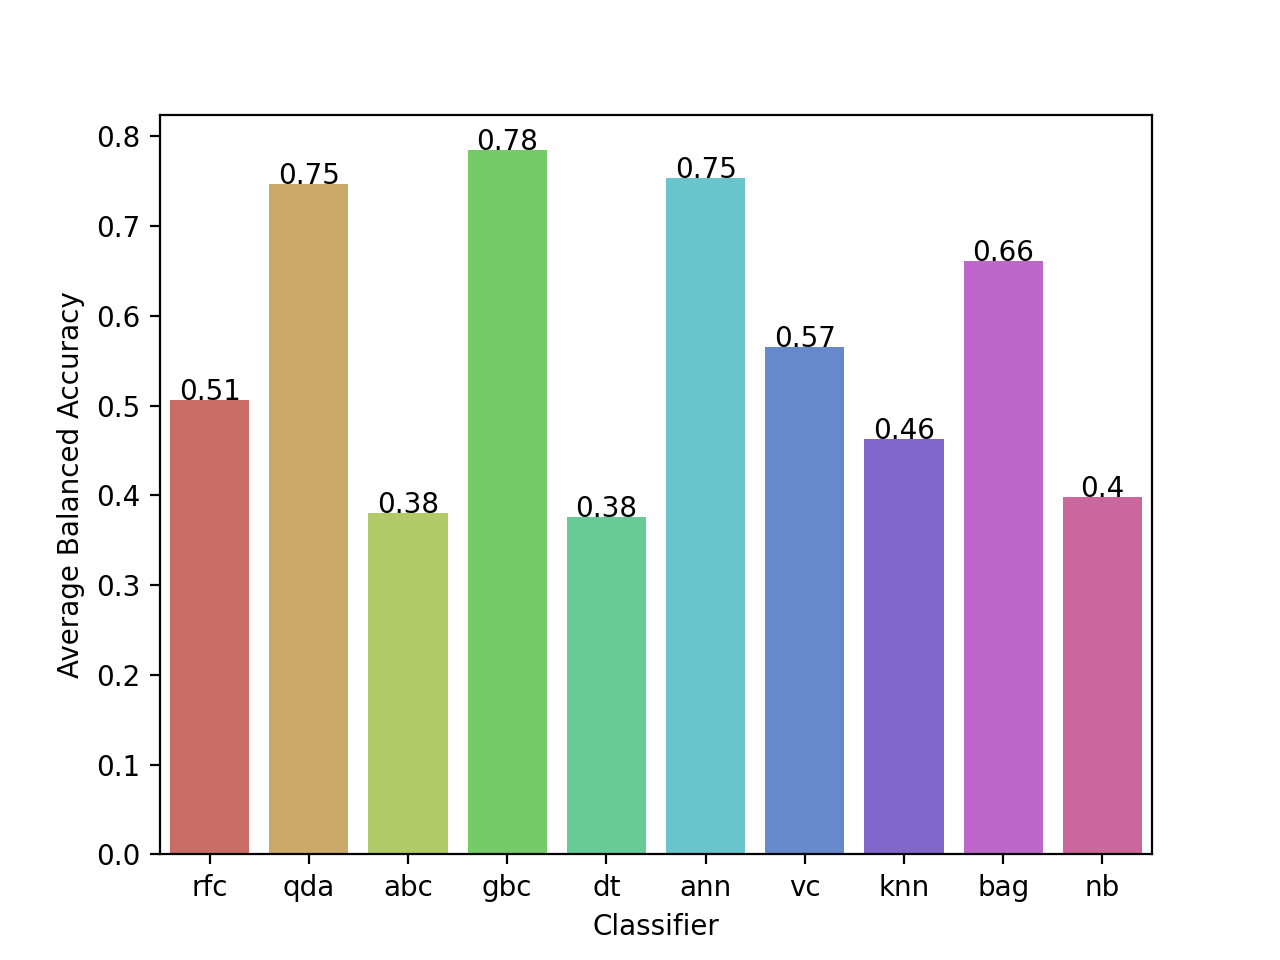
\includegraphics[width=\textwidth]{opt_grid_bar.png}
    \caption{Average prediction accuracy of coverages where a model performed well. 
    GBC had the highest average accuracy, but had a very small coverage.}
    \label{fig:grid_opt_graph}
\end{figure}

\par
Figure~\ref{fig:grid_opt_graph} represents the average prediction accuracy across all coverages where a model was "best fit".
What this graph shows is that the Random Forest Classifier had an average prediction rate of 51\% across coverages.
This is fairly consistent with what was expected. 
The models only trained on data contained within a coverage, which limited the training and fitting for models. 
However, other models did not suffer from this on average.
This suggests that some coverages can be broader than others.
For example, coverages where the random forest classifier performed well, may yield a higher accuracy if they are decreased or reformed.
Other coverages can be increased in size and potentially yield similar results.

% \begin{table}[htp]
%     \centering
%     \begin{tabular}{|c c c|}
%         \hline
%         \textbf{Model} & \textbf{Average F1 Score} & \textbf{Mean Balanced Accuracy} \\
% 		\hline
% 		Grid Optimized Model Injector & 0.83 & 0.862 \\
% 		\hline
%     \end{tabular}
%     \label{table:GRID_OPT_RESULTS}
%     \caption{Grid Optimized Model Injector Results}
% \end{table}

\par
The evidence supports the theory that a \ac{ML} model can be chosen based on geospatial location.
Future work may include investigating the appropriate feature sets, coverage boundaries, depth boundaries, parameters, and metrics based on geophysical location.
For example, volcanic activity creates new land.
This activity has a causal relationship to bathymetry, but volcanic activity at a specific point may not affect the bathymetry at a potential antipodal point.
This is another example that the coverage boundaries are potentially a naive selection choice.
It is possible that choosing models by performance across depth boundaries proves to be a better selector.
%Extending off the research preformed in \cite{jena2012prediction} these metrics allow the selection of the best preforming model.
%This is where I define what happens after the appropriate coverages have been found.
\par
In theory, this injection will allow each model to perform to its optimum.
Each coverage highlights distinct characteristics that will produce a better decision boundary.
These coverages are simple partitions of the world, but could be extended in future work to optimize the selection.
% Reconsider this sentence....



%Maybe here I can have a table show casing the preformance of models or possibly statistics about the coverages??
%It will be intersting to see what has preformed better across the globe
%Also is intersting to see which models have preformed best overall.

\subsection{General Discussion}
The predictions made in this work are based on predicted bathymetry.
Even with an 85\% prediction rate, these models are not able to compete with physics models.
The experiments in this work do show that there are accuracy gains to be achieved with model selection.
Figure~\ref{fig:coveragegrid} gives evidence that there is not a best fit model for predicting bathymetry globally.
This means that an ensemble of some kind, combining models based on geospatial location, feature sets, or any other unknown parameter, will likely yield better results.

The experiments in this work provide evidence for optimal model selection with regards to predicting global bathymetry.
It is reasonable to assume that selecting a model with a decision function will produce better predictions.
Identifying the optimal decision function will help to explain why different models perform better or worse over a coverage.
The Grid Optimized Model Injector shows that a simple geospatial decision function can be used to improve a theoretical prediction accuracy.

Selecting a model with a decision function is a novel concept for predicting bathymetry.
The evidence supports that this will yield better results.
An effective decision function could be something similar to the geospatial cache utilized in the Model Injector, or a decision based on selected features, or discovering optimal polygon coverages.
In theory, optimizing the predictor for a region extend to utilizing both \ac{ML} models and physics models.
This results in the most accurate model making predictions across the globe, therefore rasing accuracy globally.

    \section{Future Work}
\setlength{\parindent}{10ex}
There are many interesting avenues to explore from the research performed in this work.
A first avenue will be to perform the experiments in this work at a higher spatial resolution.
This work used a 2 minute spatial grid for representing all features and bathymetry.
A 2 minute grid was used for the memory and size advantages.
Allowing the computations and models to be fit on a pedestrian work station.
Modern datasets for bathymetry are often represented in higher resolution grids.
Naturally, the results will scale to the higher resolution, but testing and reporting the results will be necessary.

\par
Another interesting avenue will be to explore selecting features based on geophysical location.
This could be tested by performing feature selection on the models across different coverages of the globe.
A simple genetic algorithm could be run for each model.
The resulting features will then be used to for training and the best performing model will be selected with the optimum features.
This experiment will eliminate features that do not locally support the model while highlighting the locally important features.

\par
The same approach to feature selection could be taken to parameter tuning.
Running a similar genetic algorithm to tune optimum parameters could potentially yield better results.
Searching for optimal coverages is also a great avenue to explore.

\par 
Defining the best decision function for model selection is also a worthy investment.
The core experiment in this project used a naive spatial boundary for selecting models.
However, it is possible that geographic features were primary contributors to model success.
Identifying several model selection functions and finding a optimal function will allow for conclusions to be drawn in regards to model success.

\par
Finally, this work was preformed using predicted bathymetry from the ETOPO dataset.
As already stated, this was done in order to prove the viability of the models.
Not to prove the accuracy could be greater than a \ac{EGM}.
However, this is a experiment that can be executed.
Training these models against true bathymetry and comparing the metrics to existing \ac{EGM}s will give a indication of ability to predict bathymetry.
    \section{Conclusion}
\setlength{\parindent}{10ex}
This study experimented with the viability of a \ac{ML} model for predicting global bathymetry.
Using predicted bathymetry and ocean features as training data the models were fit and analyized.
This work concluded there is not a best fit model or method for predicting bathymetry.
Using dynamic selection techniques to optimize across geophysical locations will lead to stronger models.
This was shown using a simple model selection to boost the performance of classifiers.
Analyizing the research performed in this paper it can be conjectured that combining optimized \ac{ML} models with accurate \ac{EGM}s could lead to highly accurate prediction models.

    \section{Acronyms}
    \begin{acronym}
    \acro{MBES}{Multi-Beam Echo Sounder}
    \acro{SBES}{Single Beam Echo Sounder}
    \acro{EGM}{Earth Gravitational Model}
    \acro{SDB}{Satellite-Derived Bathymetry}
    \acro{NAVO}{Naval Oceanographic Office}
    \acro{GEBCO}{General Bathymetric Chart of the Oceans}
    \acro{JAMSTEC}{Japan Agency for MarineEarth Science and Technology}
    \acro{NOAA}{National Oceanic and Atmospheric Administration}
    \acro{NGA}{National Geospatial Agency}
    \acro{RMSE}{Root Mean Square Error}
    \acro{ASW}{Anti Submarine Warfare}
    \acro{MIW}{MIne Warfare}
    \acro{ML}{Machine Learning}
    \acro{CRS}{Coordinate Reference System}
    \acro{ETOPO}{Earth TOPOgraphy}
    \acro{NGDC}{National Geophysical Data Center}
    \acro{API}{Application Programming Interface}
    \acro{ANN}{Artificial Neural Network}
    \acro{RFC}{Random Forest Classifier}
\end{acronym}
    \printbibliography
\end{document} 